\documentclass[14pt]{mmcs_article}
\usepackage[russian]{babel}
\usepackage{amsmath, amsthm, amsfonts, amssymb}

%\graphicspath{{images/}}%путь к рисункам

\begin{document}

%см. РЕКОМЕНДАЦИИ ПО ОФОРМЛЕНИЮ
%И ПРЕДСТАВЛЕНИЮ КУРСОВЫХ И ВЫПУСКНЫХ %КВАЛИФИКАЦИОННЫХ РАБОТ СТУДЕНТОВ ИНСТИТУТА %МАТЕМАТИКИ, МЕХАНИКИ И КОМПЬЮТЕРНЫХ НАУК


% ----------------------------------
% Внимание!
% Изменяйте только строки, перед которыми стоят знаки комментариев
% ----------------------------------

\thispagestyle{empty}
\begin{singlespacing}
\begin{center}

МИНОБРНАУКИ РОССИИ\\ [12pt]
Федеральное государственное автономное образовательное\\
учреждение высшего образования\\
<<Южный федеральный университет>>

\vspace{\baselineskip}
Институт математики, механики\\
и компьютерных наук им.~И.\,И.~Воровича

\vspace{\baselineskip}
% Название выпускающей кафедры
Кафедра алгебры и дискретной математики

\vfill
% Фамилия Имя Отчество студента
\textbf{Иванов Иван Сергеевич}

\vspace{\baselineskip}
%НАЗВАНИЕ РАБОТЫ должно полностью соответствовать
% приказу по ЮФУ (для выпускных квалификационных работ)
{\bf НАЗВАНИЕ РАБОТЫ, \\
РАЗБИТОЕ ПРИ НЕОБХОДИМОСТИ \\
НА НЕСКОЛЬКО СТРОК }

\vspace{15mm}
ВЫПУСКНАЯ КВАЛИФИКАЦИОННАЯ РАБОТА\\
по направлению подготовки\\
% Направление обучения
% раскомментируйте нужную строчку
02.03.02~-- Фундаментальная информатика и информационные технологии
% 01.03.01~-- Математика
% 01.03.02~-- Прикладная математика и информатика
% 01.03.03~-- Механика и математическое моделирование 	


\vspace{10mm}
\textbf{Научный руководитель~--}\\
% указать данные о руководителе
% должность, степень, звание Фамилия Имя Отчество
проф., д.\,ф.-м.\,н. Сергеев Петр Сергеевич

\vspace{15mm}

\noindent
% указать Фамилию и инициалы 
% заведующего выпускающей кафедры
\begin{flushleft}
Допущено к защите:\\
заведующий кафедрой \underline{\hspace*{65mm}} Сидоров С.\,С.
\end{flushleft}




\vfill
% год!
Ростов-на-Дону -- 2020

\end{center}

\singlespacing
\end{singlespacing} 

\renewcommand{\contentsname}{Оглавление}

\tableofcontents

%=======================
\newpage
\addcontentsline{toc}{section}{Постановка задачи}

\section*{Постановка задачи}


В постановке задачи коротко (по пунктам) указывается, что необходимо сделать в рамках работы. Раздел <<Постановка задачи>> должен соответствовать заданию на курсовую или выпускную квалификационную работу, подписанному научным руководителем.


%=======================
\newpage
\addcontentsline{toc}{section}{Введение}
\section*{Введение}

В описании современных стандартов передачи данных много внимания уделено контролю за ошибками, неизбежно возникающими в любом канале связи. В теории кодирования применяют много различных подходов к проблеме коррекции подобных ошибок. Обычно для этого вместе с последовательностью данных передают последовательность проверочных битов, которые позволяют обнаружить и даже исправить ошибочно переданные сигналы.

Каждому проверочному биту соответствует набор информационных битов, в соответствии с которыми вычисляется его значение. От того, как задано это соотношение, сильно зависит эффективность процесса передачи данных, поэтому целесообразно искать алгоритмы, максимально эффективно соотносящие поток информации с данными для проверки.

Методы построения таких соотношений, используемые в крупных компаниях, попадают под соглашения о неразглашении, поэтому широко известны только методы, связанные с полным перебором возможных матриц.

Далее мы рассмотрим подходы к решению данной задачи, основанные на рассмотрении графов с определённой структурой.

%=======================
\newpage
\section{Основные понятия и утверждения}\label{dsfs}

Определение 1. \textsl{Графом Таннера} будем называть двудольный неориентированный граф.

Вершины из одной доли графа Таннера соответствуют информационным битам, а вершины из другой ~--- проверочным. Вершины из этих долей называют \textsl{информационными} и \textsl{проверочными} соответственно. Рёбра же определяют взаимосвязь между этими двумя потоками данных.

Определение 2. \textsl{Обхватом графа} называют длину его минимального цикла.

Отметим, что обхват любого графа Таннера является чётным.

Известно, что на практике для кодирования эффективнее использовать графы с большим обхватом.

Определение 3. Граф Таннера называется \textsl{(m, n)-регулярным}, если степень каждой проверочной вершины равна m, а степень каждой информационной вершины равна n.

Определение 4. Будем называть граф Таннера \textsl{почти (3, n)-регулярным}, если большая часть информационных вершин имеет степень 3, а степень остальных не меньше двух.

На практике обычно используют (3, n)-регулярные или почти (3, n)-регулярные графы.

%=======================
\newpage
\section{Графы с регулярной структурой}

\subsection{Определение}

Графом с регулярной структурой, будем называть двудольный граф, который сотоит из заданного количества одинаковых компонент, между которыми строятся дуги таким образом, что граф изоморфен сам себе по отображению, циклически смещающему все вершины $i$-той компоненты в аналогичные вершины $i + 1 \pmod K$-той компоненты, где $K$ ~--- общее количество компонент в графе.

%TODO починить стрелку 
Граф с регулярной структурой задаётся четвёркой $\langle c, i, K \in \mathbb{N}, f: \mathbb{Z} \rightarrow \{ \mathbb{Z} \times \mathbb{N} \} \rangle$, где $c$ ~--- это количество проверочных вершин в компоненте, $i$ ~--- количество информационных вершин в компоненте, $K$ ~--- количество компонент, а $f$ ~--- отображение, по которому строятся дуги. Оно сопоставляет номера проверочных вершины внутри компоненты в относительные номера компонент и номеры информационных вершин внутри компонент, с которыми связана дуга.

На рис. \ref{stud:fig:1} изображён граф с регулярными структурами, заданный четвёркой $\langle 1, 2, 4, f: f(1) = \{ (0, 1), (0, 2), (-1, 2), (1, 1) \} \rangle$

\begin{figure}[H]
  \centering
  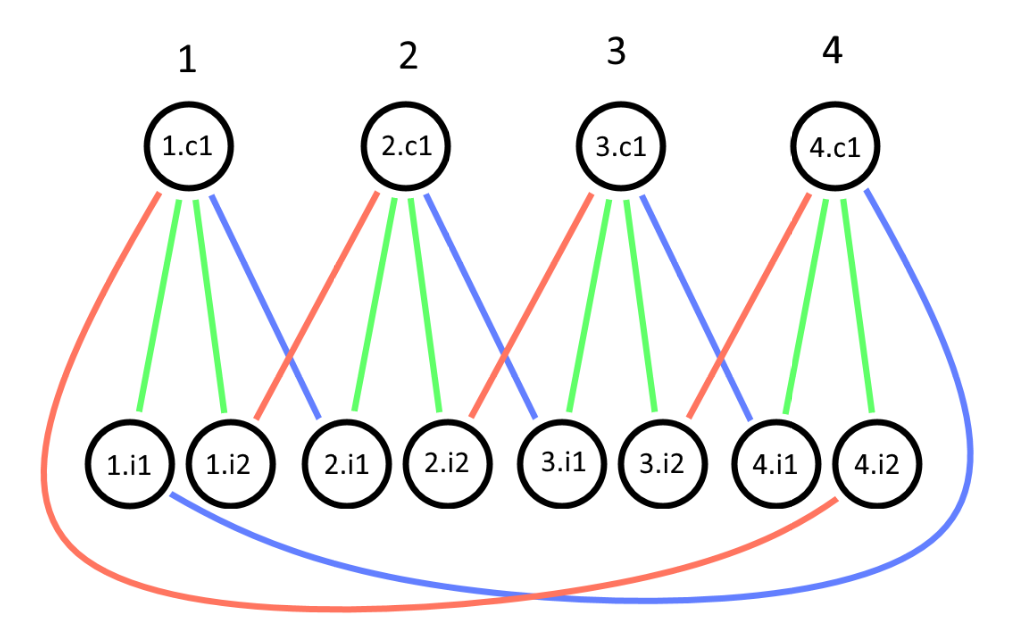
\includegraphics[scale=0.4]{Fig_1.png}
  \caption{ Граф с регулярной структурой. Компоненты пронумерованы от 1 до 4. Вершины помечены в формате \{номер компонетны\}.\{i, если вершина информационная, с, если проверочная\}\{номер вершины\} }\label{stud:fig:1}
\end{figure}

При анализе таких графов можно опустить параметр $K$, считая его достаточно большим, а затем при использовании подобрать его исходя из практических требований к размеру графа. Поэтому далее будем говорить о том, что регулярный граф задаётся тройкой $(c, i, f)$.

\subsection{Представление графов с регулярной структурой}

Тройку $\langle c, i, f \rangle$, которой задаётся граф с регулярной структурой, можно наглядно изобразить в виде компоненты, в которой проведены дуги проведены в соответствующие информационные вершины в этой же самой компоненте. Дуги следует пометить относительным номером компоненты, с которой она связана.

На рис. \ref{stud:fig:2} изображено подобное представление графа, соответствующего тройке $\langle 1, 2, f: f(1) = \{ (0, 1), (0, 2), (-1, 2), (1, 1) \} \rangle$

\begin{figure}[H]
  \centering
  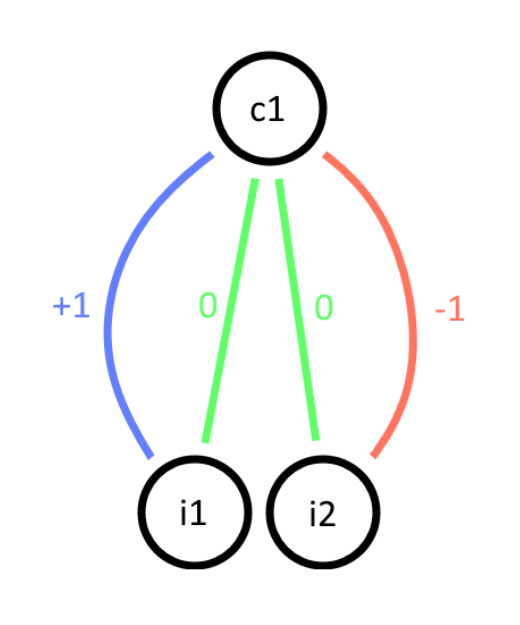
\includegraphics[scale=0.4]{Fig_2.png}
  \caption{ Упрощённое представление графа с регулярной структурой. }
  \label{stud:fig:2}
\end{figure}

\subsection{Поиск циклов в графах с регулярной структурой}

Так как основная задача при построении таких графов ~--- контроллировать длину минимального цикла, рассмотрим алгоритм поиска циклов в графе с регулярной структурой, заданном тройкой $\langle c, i, f \rangle$.

\textbf{Лемма 1.}

Если в графе с регулярными структурами есть цикл длины $t$, то через одну из проверочных вершин первой компоненты проходит цикл длины $t$.

\textbf{Доказательство.}

Любой цикл в двудольном графе проходит через какую-то проверочную вершину. Обозначим номер компоненты $d$, а индекс проверочной вершины внутри компоненты через $j$. Из определения графа с регулярными компонентами, следует, что он изоморфен сам себе по отображению, циклически сдвигающему все вершины каждой $i$-той компоненты в $i - d \pmod K$-тую компоненту. Следовательно, существует цикл длины $t$, проходящий через $j$-тую проверочную вершину первой компоненты.

\qed

Из леммы 1 следует, что чтобы показать, что минимальный цикл в графе имеет длину $t$, достаточно убедиться, что через проверочные вершины одной компоненты не проходят циклы короче, чем $t$.

В листинге \ref{stud:lst:1} приведён алгоритм поиска циклов проходящих через $j$-тую проверочную вершину. Для того, чтобы найти кратчайший цикл во всём графе нужно применить алгоритм ко всем проверочным вершинам компоненты.

\textbf{Теорема 1.}

Приведённый алгоритм находит кратчайший цикл, проходящий через заданную проверочную вершину.

\textbf{Доказательство.}

Если вершина в неком поколении $\phi$ помечена неким числом $n$, значит кратчайший путь до этой вершины в компоненте $n$ от заданной проверочной вершины равен $\phi$, так как фактически осуществляется поиск в ширину, который находит кратчайшие пути. Если существует два кратчайших пути длмны $\phi$ без общих вершин (кроме начальной и конечной) до вершины, алгоритм завершается.

Если существует кратчайший цикл длины $t$, значит в этом цикле есть вершина $v$, до которой существует два пути длины $t / 2$, в которых нет совпадающий вершин. Так как цикл кратчайший, то пути до вершины $v$ короче, чем $t / 2$ нет. Если есть два пути длины $t / 2$, у которых есть общие вершины (кроме начальной и конечной), то они образуют цикл длины, меньшей, чем $t$, следовательно таких путей нет.

Таким образом, алгоритм обязательно найдёт кратчайший цикл. \qed

\begin{lstlisting}[caption={Алгоритм поиска циклов}, label=stud:lst:1]
//   Возвращает длину самого короткого цикла, проходящего через j-тую
// проверочную вершину компоненты или -1, если циклов меньше или равных
// max-cycle не найдено
fn find-cycle(j, max-cycle) {
    // Начинаем работу с первого поколения
    generation = 1;
    //   Словарь где ключами выступают вершины и поколения,
    // а значения - множества меток.
    //   Метки соответствуют пройденному пути.
    //   Изначально j- тая проверочная вершина помечена нулём.
    labels = { (control(j), generation): { 0 } };
    для всех вершин vertex в текущем поколении {
        generation += 1;
        для всех дуг edge, соединённых с vertex {
            для всех меток label на вершине vertex
            в текущем поколении {
                next-vertex = вершина, с которой соединена дуга;
                shifted-label = label + edge.label;

                если next-vertex уже помечена shifted-label
                в одном из предыдущих поколений поколении:
                    continue;

                если next-vertex уже помечена shifted-label 
                в текущем поколении:
                    return generation * 2;
                
                пометить next-vertex shifted-label
                в текущем поколении
            }
        }
        если generation >= max-cycle / 2:
            return -1;
    }
}
\end{lstlisting}


%=======================
\newpage
\addcontentsline{toc}{section}{Заключение}
\section*{Построение графа с регулярной структурой и заданным минимальным циклом.}

%=======================
\newpage
\addcontentsline{toc}{section}{Заключение}
\section*{Заключение}


%=======================
\newpage

\addcontentsline{toc}{section}{Литература}
\renewcommand{\refname}{\centering \textbf{Литература}}


\end{document}
% ----------------------------------------------------------------


\lstset{ %
language=C++,                 % выбор языка для подсветки (здесь это С++)
basicstyle=\small\sffamily, % размер и начертание шрифта для подсветки кода
numbers=left,               % где поставить нумерацию строк (слева\справа)
numberstyle=\tiny,           % размер шрифта для номеров строк
stepnumber=1,                   % размер шага между двумя номерами строк
numbersep=5pt,                % как далеко отстоят номера строк от подсвечиваемого кода
backgroundcolor=\color{white}, % цвет фона подсветки - используем \usepackage{color}
showspaces=false,            % показывать или нет пробелы специальными отступами
showstringspaces=false,      % показывать или нет пробелы в строках
showtabs=false,             % показывать или нет табуляцию в строках
frame=single,              % рисовать рамку вокруг кода
tabsize=2,                 % размер табуляции по умолчанию равен 2 пробелам
captionpos=t,              % позиция заголовка вверху [t] или внизу [b]
breaklines=true,           % автоматически переносить строки (да\нет)
breakatwhitespace=false, % переносить строки только если есть пробел
escapeinside={\%*}{*)}   % если нужно добавить комментарии в коде
extendedchars=true,
commentstyle=\color{mygreen},    % comment style
stringstyle=\bf,
commentstyle=\ttfamily\itshape,
keepspaces=true % пробелы между русскими буквами
aboveskip=3mm,
belowskip=3mm

}


\renewcommand\NAT@bibsetnum[1]{\settowidth\labelwidth{\@biblabel{#1}}%
   \setlength{\leftmargin}{\bibindent}\addtolength{\leftmargin}{\dimexpr\labelwidth+\labelsep\relax}%
   \setlength{\itemindent}{-\bibindent+\fivecharsapprox}%
   \setlength{\listparindent}{\itemindent}
\setlength{\itemsep}{\bibsep}\setlength{\parsep}{\z@}%
   \ifNAT@openbib
     \addtolength{\leftmargin}{\bibindent}%
     \setlength{\itemindent}{-\bibindent}%
     \setlength{\listparindent}{\itemindent}%
     \setlength{\parsep}{0pt}%
   \fi
}
\renewcommand{\thesection}{\arabic{section}.}
\renewcommand{\thesubsection}{\arabic{section}.\arabic{subsection}.}
